\documentclass[ngerman, table, 9pt]{beamer}
\usetheme{metropolis}

%\usepackage[all]{hypcap}
\usepackage{colortbl}
\usepackage{scrhack}

%\usepackage{FiraSans} %% option 'sfdefault' activates Fira Sans as the default text font
%\usepackage[T1]{fontenc}
%\renewcommand*\oldstylenums[1]{{\firaoldstyle #1}}
%\usepackage[no-math]{fontspec}
\usepackage{babel}
%\usepackage[pdfborder={0 0 0}]{hyperref}
%\usepackage{amsmath}
\usepackage{adjustbox}
\usepackage{graphicx}
\usepackage[super]{nth}
%\usepackage{float}
%\usepackage{amsfonts}
%\usepackage{textcomp}

% REFERENCE: https://www.ctan.org/tex-archive/macros/latex/contrib/drawstack
\usepackage[nocolor]{drawstack}
\tikzstyle{occupiedcell}=[fill=white!70!black, draw=black]

\usepackage[backend=biber,style=alphabetic,sorting=ynt]{biblatex}
\addbibresource{deps/paper/bibliography.bib}


\setmainfont{Fira Sans}
\setsansfont{Fira Sans}
\setmonofont[Scale=MatchLowercase]{JetBrains Mono NL}

% \setlength{\parindent}{0pt}
\setlength{\parskip}{4pt}

\usepackage[autostyle]{csquotes}

\newcommand{\RNum}[1]{\uppercase\expandafter{\romannumeral #1\relax}}
\newcommand{\encircle}[1]{\raisebox{.5pt}{\textcircled{\raisebox{-.8pt} {\footnotesize#1}}}}
\newcommand{\TODO}[1]{\textcolor{red}{\textbf{TODO: #1}}}
\newcommand{\rushCommit}{\ignorespaces\texttt{\input "|git -C ./deps/rush rev-parse --short HEAD"}\unskip}
\newcommand{\tokei}[1]{\input "|python3 tokei.py #1"}
\newcommand{\riscv}{RISC\babelhyphen{nobreak}V}

\newcommand{\qVerb}[2][]{\enquote{\Verb[#1]{#2}}}
\newcommand{\VerbCmd}[2][]{\Verb[commandchars=\\\{\}, #1]{#2}}
\newcommand{\qVerbCmd}[2][]{\qVerb[commandchars=\\\{\}, #1]{#2}}
\newcommand{\reg}[1]{\VerbCmd{\%#1}}
\newcommand{\qreg}[1]{\qVerbCmd{\%#1}}


% \setcounter{tocdepth}{3}% Include \subsubsection in ToC

\definecolor{DarkTeal}{HTML}{23373b}
\newcommand{\cemph}[1]{\textcolor{mLightBrown}{#1}}

\newcounter{chapter}
\setcounter{chapter}{1}

\newcommand{\scite}[2][]{{\footnotesize\cite[#1]{#2}}}


\newcommand{\Larrow}[1]{
	\begin{tikzpicture}[triangle/.style={-{Triangle[width=\the\dimexpr1.8\pgflinewidth,length=\the\dimexpr0.8\pgflinewidth]}}]
		\draw[line width=9pt,triangle](0,0) -- node[anchor=south, yshift=.15cm] {\footnotesize #1} (1.4,0);
	\end{tikzpicture}
}

\newcommand{\Darrow}[1]{
	\begin{tikzpicture}[triangle/.style={-{Triangle[width=\the\dimexpr1.8\pgflinewidth,length=\the\dimexpr0.8\pgflinewidth]}}]
		\draw[line width=9pt,triangle](0,0) -- node[anchor=west, xshift=.15cm] {\footnotesize #1} (0, -1.4);
	\end{tikzpicture}
}


\input{preamble/tabularx}
\input{preamble/drawstack}

\input{|"lirstings include-tex"}
\captionsetup{labelformat=empty}
% Set `deps/rush` as path prefix in all lirstings, is ignored for files under other directories
\NewCommandCopy{\oldLirsting}{\Lirsting}
\renewcommand{\Lirsting}[2][]{\oldLirsting[path prefix={deps/rush},vspace=0pt,#1]{#2}}

\input{preamble/tikz}

\title{Die Umwandlung von Quelltext in Maschinensprache}
\date{17. Mai 2023}
\author{Silas Groh, Mik Müller}
\institute{Carl-Fuhlrott-Gymnasium}

\titlegraphic{\rushlogo{y=0.80pt, x=0.80pt, yscale=-0.17, xscale=0.17}}

\begin{document}
\begin{frame}
	\titlepage
\end{frame}

% chktex-file -2
% LTeX: language=de-DE

\section{Einstieg \& Motivation}
\begin{frame}{Einstieg \& Motivation}
	\begin{itemize}
		\item Programme werden in speziellen Sprachen verfasst
		\item Vorteile eines hohen Abstraktionsgrades
	\end{itemize}
\end{frame}

\begin{frame}{Einstieg \& Motivation}
	\begin{figure}[h]
		\begin{minipage}{.32\textwidth}
			\begin{center}
				\centering
				\centerline{\includegraphics[width=.5\textwidth]{assets/google_icon_construction.png}}
				{\small Erweiterbarkeit \& Reperatur}
			\end{center}
		\end{minipage}
		\pause
		\hfill
		\begin{minipage}{.32\textwidth}
			\begin{center}
				\centerline{\includegraphics[width=.5\textwidth]{assets/google_icon_deployed_code.png}}
				{\small Portabilität \& Platformunabhängigkeit}
			\end{center}
		\end{minipage}
		\pause
		\hfill
		\begin{minipage}{.32\textwidth}
			\begin{center}
				\centerline{\includegraphics[width=.5\textwidth]{assets/google_icon_speed.png}}
				{\small Geschwindigkeit \& Einfachheit }
			\end{center}
		\end{minipage}
	\end{figure}
\end{frame}

\begin{frame}{Zentrales Problem}
	\begin{minipage}{.35\textwidth}
		\Lirsting[float=H, fancyvrb={frame=none, fontsize=\small}]{deps/paper/listings/simple.rush}
	\end{minipage}%
	\hfill
	\Larrow{
		\begin{minipage}{0.9cm}
			Vorgang
		\end{minipage}
		\begin{minipage}{5mm}
			\includegraphics[width=3.5mm]{assets/google_icon_settings.png}
		\end{minipage}
	}
	\hfill
	\begin{minipage}{.34\textwidth}
		% \Lirsting[float=H, fancyvrb={frame=none, fontsize=\small}, ranges={1-10}]{listings/rush_simple.hexdump}
		\centerline{\includegraphics[width=.5\textwidth]{assets/google_icon_question_mark.png}}
	\end{minipage}

	\begin{itemize}
		\item Programme sollten \cemph{einfach} zu schreiben sein
		\item[\Rightarrow] Ein Computer muss diese jedoch auch \cemph{einfach} verarbeiten
	\end{itemize}
\end{frame}

\begin{frame}{Methoden zur Programmausführung}
	\begin{itemize}
		\item Man unterscheidet zwischen \cemph{Compilern} und \cemph{Interpretern}
		\item Compiler: übersetzt das Programm in ein Zielformat
		\item Interpreter: führt das Programm direkt aus (keine Übersetzung)
	\end{itemize}
\end{frame}

\begin{frame}{Interpreter}
	\hfill
	\begin{minipage}{.35\textwidth}
		\begin{center}
			\Lirsting[float=H, fancyvrb={frame=none, fontsize=\small}]{deps/paper/listings/simple.rush}
		\end{center}
	\end{minipage}%
	\Larrow{
		\begin{minipage}{1.3cm}
			Ausführung
		\end{minipage}
		\begin{minipage}{5mm}
			\includegraphics[width=3.5mm]{assets/google_icon_settings.png}
		\end{minipage}
	}
	\hfill
	\begin{minipage}{.35\textwidth}
		\centering
		{\LARGE Exit code: 5}
	\end{minipage}
	\hfill

	\begin{itemize}
		\item Python, Javascript, PHP, usw.
		\item Keine Übersetzung notwending
		\item[\Rightarrow] Interpretiert den Syntaxbaum direkt
	\end{itemize}
\end{frame}

\begin{frame}{Compiler}
	\hspace{.8cm}
	\begin{minipage}{.35\textwidth}
		\begin{center}
			\Lirsting[float=H, fancyvrb={frame=none, fontsize=\small}]{deps/paper/listings/simple.rush}
		\end{center}
	\end{minipage}%
	\Larrow{
		\begin{minipage}{1.45cm}
			Übersetzung
		\end{minipage}
		\begin{minipage}{5mm}
			\includegraphics[width=3.5mm]{assets/google_icon_settings.png}
		\end{minipage}
	}
	\hspace{1.9cm}
	\begin{minipage}{.26\textwidth}
		\Lirsting[float=H, fancyvrb={frame=none, fontsize=\small}, ranges={1-10}]{listings/rush_simple.hexdump}
	\end{minipage}
	\hfill

	\begin{itemize}
		\item Rust, C, Go, usw.
		\item Zusätzlicher Prozess
		\item Umwandlung in ein anderes Format
		\item[\Rightarrow] Muss vor der Ausführung stattfinden
	\end{itemize}
\end{frame}

\section{Die Programmiersprache \enquote{rush}}

\begin{frame}{Fakten über rush}
	\begin{figure}[h]
		\flushleft
		\hspace{.15cm} \rushlogo{y=0.80pt, x=0.80pt, yscale=-0.15, xscale=0.15}
		\vspace{.2cm}
	\end{figure}
	\begin{itemize}
		\item ca.\ vier Monate intensive Entwicklung
		\item \rushCountCommits~Git Commits
		\item \tokei{./deps/rush} Zeilen Programmtext\footnote{Leerzeilen und Kommentare werden nicht gezählt.} in Git Commit `\rushCommit'
	\end{itemize}
\end{frame}

\begin{frame}{Inhalte des Projektes}
	\begin{itemize}
		\item Lexer
		\item Parser
		\item Semantikanalyse
		\item zwei Interpreter
		\item ein Transpiler
		\item vier Compiler
	\end{itemize}
\end{frame}

\begin{frame}{Fähigkeiten von rush}
	\pdfpcnote{
		1. Schleife \\
		2. while-Schleife \\
		3. for-Schleife \\
		4. if-Verzweigung \\
		5. Funktionsdefinition \\
		6. infix-Ausdruck \\
		7. praefix-Ausdruck \\
		8. Variablendefinition \\
		9. Typumwandlung \\
	}

	\begin{table}[h]
		\rowcolors{2}{gray!15}{}
		\begin{tabular}{p{5.2cm}|p{5.2cm}}
			\rowcolor{gray!25} Bezeichnung & Beispiel                                                 \\
			\hline
			Schleife                       & \LirstInline{rush}{loop {  }}                     \pause \\
			\enquote{while}-Schleife       & \LirstInline{rush}{while x < 5 {  }}              \pause \\
			\enquote{for}-Schleife         & \LirstInline{rush}{for i = 0; i < 5; i += 1 {  }} \pause \\
			\enquote{if}-Verzweigung       & \LirstInline{rush}{if true {  } else {  }}        \pause \\
			Funktionsdefinition            & \LirstInline{rush}{fn foo(n: int) {  }}           \pause \\
			Infix-Ausdruck                 & \LirstInline{rush}{1 + n; 5 ** 2}                 \pause \\
			Präfix-Ausdruck                & \LirstInline{rush}{!false; -n}                    \pause \\
			Variablendefinition            & \LirstInline{rush}{let mut answer = 42}           \pause \\
			Typumwandlung                  & \LirstInline{rush}{42 as float}                          \\
		\end{tabular}
	\end{table}
\end{frame}

\begin{frame}{Datentypen in rush}
	\pdfpcnote{
		1. int \\
		2. float \\
		3. bool \\
		4. char \\
		5. unit \\
		6. never \\
	}

	\begin{table}[h]
		\rowcolors{2}{gray!15}{}
		\begin{tabular}{p{5.2cm}|p{5.2cm}}
			\rowcolor{gray!25} Bezeichnung & Instanziierung einer Variable                   \\
			\hline
			\qVerb{int}                    & \LirstInline{rush}{let a: int = 0;}      \pause \\
			\qVerb{float}                  & \LirstInline{rush}{let b: float = 3.14;} \pause \\
			\qVerb{bool}                   & \LirstInline{rush}{let c: bool = true;}  \pause \\
			\qVerb{char}                   & \LirstInline{rush}{let d: char = 'a';}   \pause \\
			\qVerb{()} oder \enquote{Unit} & \LirstInline{rush}{let e: () = main();}  \pause \\
			\qVerb{!} oder \enquote{Never} & \LirstInline{rush}{let f = exit(42);}           \\
		\end{tabular}
	\end{table}
\end{frame}

\begin{frame}{Berechnung von Fibonaccizahlen in rush}
	\begin{minipage}{.6\textwidth}
        \Lirsting[float=H, fancyvrb={frame=none}]{deps/paper/listings/fib.rush}
	\end{minipage}
	\begin{minipage}{.3\textwidth}
		\begin{align*}
			f_n & = f_{n-2} + f_{n-1} & ; n \ge 3 \\
			f_1 & = f_2 = 1
		\end{align*}
	\end{minipage}
\end{frame}

\newcommand{\fadeout}[1]{\textcolor<2>{black!30}{#1}}
\begin{frame}{Umfang der einzelnen Komponenten}
	\pdfpcnote{
		- Uebersicht von rush Komponenten und den jeweiligen Zeilen an Programmtext \\
		- leere Zeilen und Kommentare werden nicht mitgezaehlt \\
        \\
        --- \\
        \\
        - Fokus auf Interpreter: das kleinste Teilprojekt -> simpel \\
        - Fokus auf LLVM: durchschnittlich \\
        - Fokus auf x64: Das groesste Teilprojekt -> komplex \\
	}

	\begin{table}[h]
		\centering
		\rowcolors{2}{gray!15}{}
		\begin{tabular}{p{5.2cm}|p{5.2cm}}
			\rowcolor{gray!20} Komponente   & Zeilen Programmtext                                       \\
			\hline
			\fadeout{Lexer / Parser}        & \fadeout{\tokei{./deps/rush/crates/rush-parser}}          \\
			Tree-walking Interpreter        & \tokei{./deps/rush/crates/rush-interpreter-tree}          \\
			\fadeout{VM Compiler / Runtime} & \fadeout{\tokei{./deps/rush/crates/rush-interpreter-vm}}  \\
			\fadeout{WASM Compiler}         & \fadeout{\tokei{./deps/rush/crates/rush-compiler-wasm}}   \\
			LLVM Compiler                   & \tokei{./deps/rush/crates/rush-compiler-llvm}             \\
			\fadeout{RISC-V Compiler}       & \fadeout{\tokei{./deps/rush/crates/rush-compiler-risc-v}} \\
			x64 Compiler                    & \tokei{./deps/rush/crates/rush-compiler-x86-64}           \\
		\end{tabular}
	\end{table}
\end{frame}

\begin{frame}{Stufen der Übersetzung~\scite[S.~6--7]{wirth_compiler_construction_2005} \TODO{MAYBE DELETE}}
	\hspace{0pt} % This is somehow required
	\vfill
	\begin{figure}[h]
		\begin{adjustbox}{max totalsize={\textwidth}{!},center}
			\begin{tikzpicture}[node distance=1cm, inner sep=3mm]
				\node (lexical_analysis) [rec, minimum height=1.5cm] {Lexikalische Analyse};
				\node (syntactic_analysis) [rec, right=of lexical_analysis, align=center, minimum height=1.5cm] {Syntaxanalyse};
				\draw [arrow] (lexical_analysis) -- (syntactic_analysis);
				\node (semantic_analysis) [rec, right=of syntactic_analysis, align=center, minimum height=1.5cm] {Semantische\\Analyse};
				\draw [arrow] (syntactic_analysis) -- (semantic_analysis);
				\node (codegen) [rec, right=of semantic_analysis, minimum height=1.5cm] {Code-Erzeugung};
				\draw [arrow] (semantic_analysis) -- (codegen);
			\end{tikzpicture}
		\end{adjustbox}
	\end{figure}
	\vfill
	\begin{figure}[h]
		\begin{adjustbox}{max totalsize={\textwidth}{!},center}
			\begin{tikzpicture}[node distance=3mm and 1cm, inner sep=3mm]
				\node (syntactic_analysis_text) [inner sep=0] {Syntaxanalyse};
				\node (lexical_analysis) [rec, below=of syntactic_analysis_text] {Lexikalische Analyse};
				\node (syntactic_analysis) [rec, fit={(syntactic_analysis_text) (lexical_analysis)}] {};
				\node (semantic_analysis) [rec, right=of syntactic_analysis] {Semantische Analyse};
				\draw [arrow] (syntactic_analysis) -- (semantic_analysis);
				\node (codegen) [rec, right=of semantic_analysis] {Code-Erzeugung};
				\draw [arrow] (semantic_analysis) -- (codegen);
			\end{tikzpicture}
		\end{adjustbox}
	\end{figure}
	\vfill
\end{frame}

% LTeX: language=de-DE
\section{Lexikalische \& Syntaktische Analyse}

\begin{frame}{Etappen der Übersetzung: Semantische Analyse}
	\begin{figure}[h]
		\begin{adjustbox}{max totalsize={\textwidth}{!},center}
			\begin{tikzpicture}[node distance=1cm, inner sep=3mm]
				\node (lexical_analysis) [rec, minimum height=1.5cm, fill=gray!25] {Lexikalische Analyse};
				\node (syntactic_analysis) [rec, right=of lexical_analysis, align=center, minimum height=1.5cm, fill=gray!25] {Syntaxanalyse};
				\draw [arrow] (lexical_analysis) -- (syntactic_analysis);
				\node (semantic_analysis) [rec, right=of syntactic_analysis, align=center, minimum height=1.5cm] {Semantische\\Analyse};
				\draw [arrow] (syntactic_analysis) -- (semantic_analysis);
				\node (codegen) [rec, right=of semantic_analysis, minimum height=1.5cm] {Code-Erzeugung};
				\draw [arrow] (semantic_analysis) -- (codegen);
			\end{tikzpicture}
		\end{adjustbox}

		\scite[S.~6--7]{wirth_compiler_construction_2005}
	\end{figure}
\end{frame}

\begin{frame}{Lexikalische \& Syntaktische Analyse \TODO{DELETE}}
	\begin{itemize}
		\item Gruppieren des Programmtextes in Tokens
		\item Analyse der Syntax des Programms
		\item Erzeugung eines abstrakten Syntaxbaums
		\item Festlegen der formalen Regeln in Form einer Grammatik
	\end{itemize}

	\centering
    \Lirsting[float=H, fancyvrb={fontsize=\small}, ranges={1-5:33, _5:66-5}, caption={Ein Beispiel für eine kontextfreihe Grammatik (EBNF)}]{listings/grammar.ebnf}
\end{frame}

\begin{frame}{Abstrakter Syntaxbaum \TODO{DELETE}}
	\begin{figure}[h]
		\begin{minipage}{.35\textwidth}
			\centering
			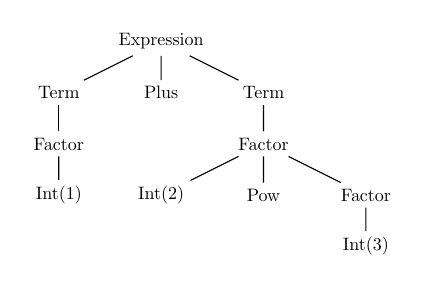
\begin{tikzpicture}[level distance=1cm, sibling distance=2cm, scale=.65, transform shape]
				\node {Expression}
				child {node {Term}
						child {node {Factor}
								child {node {\Verb{Int(1)}}}}}
				child {node {\Verb{Plus}}}
				child {node {Term}
						child {node {Factor}
								child {node {\Verb{Int(2)}}}
								child {node {\Verb{Pow}}}
								child {node {Factor}
										child {node {\Verb{Int(3)}}}}}};
			\end{tikzpicture}
		\end{minipage}
		\hfill
		\begin{minipage}{.45\textwidth}
			\begin{figure}[h]
				\centering
				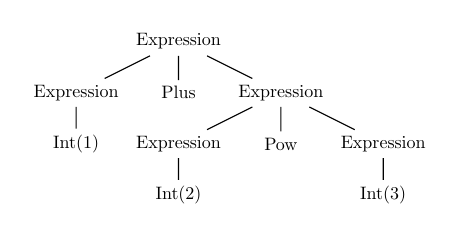
\begin{tikzpicture}[level distance=1cm, sibling distance=2cm, scale=.65, transform shape]
					\node {Expression}
					child {node {Expression}
							child {node {\Verb{Int(1)}}}}
					child {node {\Verb{Plus}}}
					child {node {Expression}
							child {node {Expression}
									child {node {\Verb{Int(2)}}}}
							child {node {\Verb{Pow}}}
							child {node {Expression}
									child {node {\Verb{Int(3)}}}}};
				\end{tikzpicture}
			\end{figure}
		\end{minipage}

        \centering
        Zwei verschiedene Syntaxbäume für \enquote{\LirstInline{rush}{1+2**3}}
	\end{figure}
\end{frame}

% LTeX: language=de-DE
\section{Semantische Analyse}

\begin{frame}{Etappen der Übersetzung: Semantische Analyse}
	\begin{figure}[h]
		\begin{adjustbox}{max totalsize={\textwidth}{!},center}
			\begin{tikzpicture}[node distance=1cm, inner sep=3mm]
				\node (lexical_analysis) [rec, minimum height=1.5cm] {Lexikalische Analyse};
				\node (syntactic_analysis) [rec, right=of lexical_analysis, align=center, minimum height=1.5cm] {Syntaxanalyse};
				\draw [arrow] (lexical_analysis) -- (syntactic_analysis);
				\node (semantic_analysis) [rec, right=of syntactic_analysis, align=center, minimum height=1.5cm, fill=gray!25] {Semantische\\Analyse};
				\draw [arrow] (syntactic_analysis) -- (semantic_analysis);
				\node (codegen) [rec, right=of semantic_analysis, minimum height=1.5cm] {Code-Erzeugung};
				\draw [arrow] (semantic_analysis) -- (codegen);
			\end{tikzpicture}
		\end{adjustbox}
		\caption{Etappen der Übersetzung: Semantische Analyse.}{\scite[S.~6--7]{wirth_compiler_construction_2005}}\label{fig:compilation_steps}
	\end{figure}
\end{frame}

\begin{frame}{Semantische Analyse \& Semantikregeln}
	\begin{itemize}
		\item Findet nach der Syntaxanalyse und vor der Übersetzung statt
		\item Validierung der semantischen Eigenschaften des Programms
		\item Die semantischen Regeln einer Programmiersprache werden oft mittels einer natürlichen Sprache beschrieben
		\item Für rush wurde ein Dokument erstellt, welches die meisten Semantikregeln erklärt
	\end{itemize}
\end{frame}

\begin{frame}{Beispiele für die Semantikregeln von rush}
	\begin{itemize}
		\item Jede Variable, jede Funktion und jeder Parameter besitzt einen Datentyp, der nach Definierung nicht mehr geändert werden kann
		\item Eine Funktion muss immer mit den Argumenten aufgerufen werden, die zu den Parametern passen
		\item Jeder Funktionsname muss eindeutig sein
		\item Die \qVerb{main} Funktion liefert immer den \qVerb{()} Datentyp und akzeptiert keine Parameter
		\item Jede Variable muss Definiert sein, bevor diese Verwendbar ist
		\item Logische und mathematische Operationen erfolgen nur, wenn die Operanten den selben Datentypen besitzen
		\item Eine definierte Variable \emph{sollte} verwendet werden
		\item[\ldots]
	\end{itemize}
\end{frame}

\begin{frame}{Beispiel: Invalides rush Programm}
	\begin{minipage}{.5\textwidth}
		\Lirsting[float=H, fancyvrb={frame=none}]{listings/incompatible_types.rush}
	\end{minipage}%
	\begin{minipage}{.5\textwidth}
		\Darrow{Fehlerausgabe}
	\end{minipage}
	\Lirsting[float=H, fancyvrb={frame=none, fontsize=\footnotesize}, ansi=true]{listings/generated/incompatible_types.rush.out}
\end{frame}

\begin{frame}{Beispiel 2: Invalides rush Programm}
	\begin{minipage}{.5\textwidth}
		\Lirsting[float=H, fancyvrb={frame=none}]{listings/invalid_main_fn.rush}
	\end{minipage}%
	\begin{minipage}{.5\textwidth}
		\Darrow{Fehlerausgabe}
	\end{minipage}
	\Lirsting[float=H, fancyvrb={frame=none, fontsize=\footnotesize}, ansi=true]{listings/generated/invalid_main_fn.rush.out}
\end{frame}

\begin{frame}{Beispiel 3: Warnung aufgrund einer unbenutzten Variable}
	\begin{minipage}{.5\textwidth}
		\Lirsting[float=H, fancyvrb={frame=none}]{listings/unused_var.rush}
	\end{minipage}%
	\begin{minipage}{.5\textwidth}
		\Darrow{Ausgabe}
	\end{minipage}
	\Lirsting[float=H, fancyvrb={frame=none, fontsize=\footnotesize}, ansi=true]{listings/generated/unused_var.rush.out}
\end{frame}

\begin{frame}{Semantische Analyse für rush}
	\begin{itemize}
		\item Muss in der Lage sein, ein invalides von einem validen Programm zu unterscheiden
		\item Kann zusätzlich hilfreiche Warnungen und Informationen generieren
		\item Fügt Informationen über Datentypen zu dem (vom Parser erstellten) AST hinzu
		\item Führt triviale Optimierungen der Programmstruktur durch
	\end{itemize}
\end{frame}

\begin{frame}{Hinzufügen von Informationen über Datentypen}

	\begin{figure}[h]
		\begin{adjustbox}{max totalsize={\textwidth}{!},center}
			\begin{tikzpicture}[
					tlabel/.style={pos=0.4,right=-1pt,font=\footnotesize\color{red!70!black}},
				]
				\node(left){\Verb{1 + 42 - n}}
				child { node { \Verb{1 + 42} }
						child { node { \Verb{1} } }
						child { node { \Verb{+} } }
						child { node { \Verb{42} } }
					}
				child { node  { \Verb{-} }       }
				child { node(leftm)  { \Verb{n} } };

				\node(right)[right of=left, xshift=7cm]{\Verb{43 - n}: \emph{int}}
				child { node(rightm) { \Verb{43}: \emph{int} } }
				child { node  { \Verb{-} } }
				child { node  { \Verb{n}: \emph{int} } };

				\draw[arrow, shorten >= 0.3cm, shorten <= 0.3cm, very thick] (leftm) -- node[above] {semantic} node[below] {analysis} ++ (rightm);
			\end{tikzpicture}
        \end{adjustbox}
		\caption{How semantic analysis affects the abstract syntax tree.}\label{fig:analysis_tree_conv}
	\end{figure}
\end{frame}

% LTeX: language=de-DE
\section{Tree-Walking Interpreter}

\begin{frame}{Tree-Walking Interpreter}
	\begin{itemize}
        \item \emph{Traversiert} den Syntaxbaum
		\item \emph{Interpretiert} das Programm direkt
	\end{itemize}
\end{frame}

\begin{frame}{Felder des Interpreters}
	\Lirsting[float=H, ranges={10-16}, fancyvrb={fontsize=\footnotesize}]{deps/rush/crates/rush-interpreter-tree/src/interpreter.rs}

	\begin{description}
		\item[scopes] Stack von Scopes; jeder Scope weist einem Variablennamen einen Laufzeitwert zu
		\item[functions] Zuweisung von Funktionsnamen zu einer geteilten Referenz zu dem entsprechenden Knoten im Syntaxbaum
	\end{description}
\end{frame}

\begin{frame}{Weitere Typdefinitionen}
	\begin{minipage}{0.6\textwidth}
		\Lirsting[float=H, ranges={6-13, 22-28}, fancyvrb={fontsize=\small}]{deps/rush/crates/rush-interpreter-tree/src/value.rs}
	\end{minipage}
	\hfill
	\begin{minipage}{0.35\textwidth}
		\begin{itemize}
			\item Aufzählung zum Speichern verschiedener Datentypen
			\item Verschiedene Unterbrechungen des Programmflusses
		\end{itemize}
	\end{minipage}
\end{frame}

\begin{frame}{Traversierung}
	\begin{figure}[H]
		\centering
		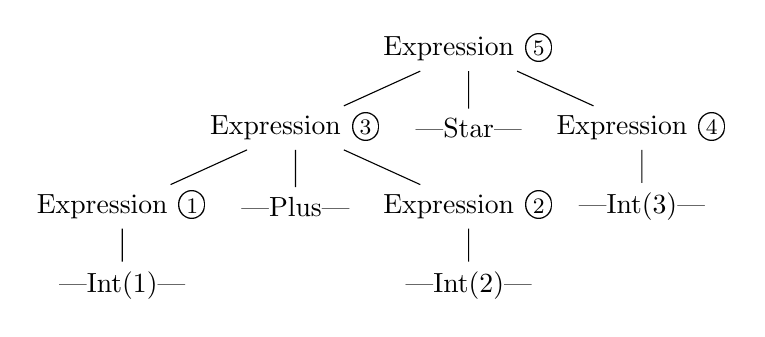
\begin{tikzpicture}[level distance=1cm, sibling distance=2.2cm]
			\node {Expression \encircle{5}}
			child {node {Expression \encircle{3}}
					child {node {Expression \encircle{1}}
							child {node {\Verb|Int(1)|}}}
					child {node {\Verb|Plus|}}
					child {node {Expression \encircle{2}}
							child {node {\Verb|Int(2)|}}}}
			child {node {\Verb|Star|}}
			child {node {Expression \encircle{4}}
					child {node {\Verb|Int(3)|}}};
		\end{tikzpicture}
        \caption{Syntaxbaum zu \enquote{\LirstInline{rush}{1 + 2 * 3}}}
	\end{figure}
\end{frame}

\begin{frame}{Effizienz}
	\begin{minipage}{0.5\textwidth}
		\Lirsting[float=H, fancyvrb={fontsize=\small}]{listings/fib.rush}
	\end{minipage}
	\hfill
	\begin{minipage}{0.45\textwidth}
		\begin{tikzpicture}
			\footnotesize
			\matrix[
			matrix of nodes,
			nodes={minimum height=3ex, draw, text width=4cm},
			row sep=-\pgflinewidth
			](stack){
            \LirstInline{rs}{call_func("fib", vec![3])} \\
			\LirstInline{rs}{visit_block(/* ... */)} \\
			\LirstInline{rs}{visit_expression(/* ... */)} \\
			\LirstInline{rs}{visit_if_expr(/* ... */)} \\
			\LirstInline{rs}{visit_block(/* ... */)} \\
			\LirstInline{rs}{visit_expression(/* ... */)} \\
			\LirstInline{rs}{visit_inifix_expr(/* ... */)} \\
			\LirstInline{rs}{visit_expression(/* ... */)} \\
			\LirstInline{rs}{visit_call_expr(/* ... */)} \\
			\LirstInline{rs}{call_func("fib", vec![2])} \\
			\dots \\
			\LirstInline{rs}{call_func("fib", vec![1])} \\
			};
			\draw[arrow] ([xshift=2.4cm]stack.north) -- ([xshift=2.4cm]stack.south);
		\end{tikzpicture}
	\end{minipage}
\end{frame}

% LTeX: language=de-DE
\section{Virtuelle Maschine}

\begin{frame}{Virtuelle Maschine}
	\begin{itemize}
		\item Meistens: Eine \emph{Virtuelle Maschine} (VM) simuliert echte Computer
		      \begin{itemize}
			      \item Display
			      \item Lautsprecher
			      \item Festplatte
			      \item \dots
		      \end{itemize}
		\item Hier: Software, die wie die CPU eines Rechners funktioniert
	\end{itemize}
\end{frame}

\begin{frame}{Wie eine CPU Programme ausführt \TODO{DELETE}}
	\begin{itemize}
		\item Die meisten Prozessoren basieren auf der \emph{von Neumann Architektur}~\scite[p.~172]{Ledin2020-yp}
		\item Eine CPU enthält nach von Neumann ein \emph{Rechenwerk}\footnote{Engl: \enquote{arithmetic logic unit} (ALU).}, \emph{Steuerwerk}\footnote{Engl: \enquote{control unit}.}, \emph{Speicherwerk}, \emph{Ein- / Ausgabewerk} und ein Bussystem~\scite[p.~172]{Ledin2020-yp}
		\item Die Programmausführung wird durch den sog. \emph{Befehlszyklus}\footnote{Engl: \enquote{fetch-decode-execute cycle}.} modelliert~\scite[pp.~208-209]{Ledin2020-yp}:
		\item[] \begin{enumerate}
				\item \textbf{Fetch} (Befehl laden): Das Steuerwerk lädt die nächste Anweisung aus dem Speicher
				\item \textbf{Decode} (Befehl dekodieren): Der Befehlscode und die Operanden werden ermittelt
				\item \textbf{Execute} (Befehl ausführen): Die zuständige Einheit im Prozessor wird verwendet, um den Befehl zu verarbeiten.
				      Beispielsweis wird das Rechenwerk für logische und mathemtische Befehle aufgerufen.
			\end{enumerate}
	\end{itemize}
\end{frame}

\begin{frame}{Übertragung der Konzepte auf die rush VM \TODO{DELETE}}
	\Lirsting[ranges={16-26}, caption={Struct Definition der VM.}, label={lst:vm_struct}, fancyvrb={fontsize=\footnotesize}, float=H, vspace=0pt]{deps/rush/crates/rush-interpreter-vm/src/vm.rs}
	\begin{itemize}
		\item \qVerb{stack}: Speicher für temporäre Werte bei komplexeren Operationen
		\item \qVerb{mem}: Anhaltender Speicher mit einer festen Größe für Variablen
		\item \qVerb{mem_ptr}: Hält den Index der letzten freien Speicherzelle in \qVerb{mem}
		\item \qVerb{call_stack}: Aufrufstapel, welcher den \emph{Befehlsähler} und den \emph{Funktionszähler} für jeden Aufruf speichert
	\end{itemize}
\end{frame}

\begin{frame}{Speicherstruktur der rush VM. \TODO{DELETE}}
	\begin{itemize}
		\item Unterscheidung zwischen zwei Arten der Adressierung
		\item \emph{relative Adressierung}: \qVerb{svari *rel[0]}
		\item \emph{absolute Adressierung}: \qVerb{svari *abs[0]}
	\end{itemize}

	\begin{figure}
		\centering
		\begin{NiceTabular}{>{\scriptsize}c}[name=Left]
			\\
			\\
			\\
			num              \\
			\Block[draw]{} 9 \\
		\end{NiceTabular}\hspace{1cm}
		\begin{NiceTabular}
			[
				first-col,
				%code-for-first-col=\ValueMinusOne{iRow},
				first-row,
				hvlines,
				colortbl-like,
				name = Right
			]
			{cc>{\scriptsize}c}
			 & cell                  & rel    & {\normalsize abs} \\
			 & a                     & $-3$   & $mp + rel = 0$    \\
			 & b                     & $-2$   & $mp + (-2) = 1$   \\
			 & c                     & $-1$   & $mp - 1 = 2$      \\
			 & d                     & $0$    & $3$               \\
			 & \cellcolor{gray!30} e & $1$    & $mp + 1 = 4$      \\
			 & \ldots                & \ldots & \ldots            \\
		\end{NiceTabular}

		\begin{tikzpicture}[overlay,remember picture]
			\draw [->] (Left-5.5-|Left-last) to [bend left] (Right-5.5-|Right-1);
			\draw [thick, dashed] (Right-4.5-|Right-5) --  node[anchor=west, xshift=-1cm, align=center] {\scriptsize memory\\ \scriptsize pointer $= 3$} ([xshift=2.5cm]Right-4.5-|Right-4);
		\end{tikzpicture}
		\caption{Speicherstruktur der rush VM.}\label{fig:rush_vm_linmem}
	\end{figure}
\end{frame}

\begin{frame}{Ein Beispielprogramm der rush VM \TODO{Delete}}
	\hspace{0pt} % This is somehow required
	\vfill
	\Lirsting[caption={Beispielprogramm der rush VM.}, fancyvrb={fontsize=\footnotesize}, float=H]{deps/paper/listings/vm_faster_instructions.s}
	\vfill
\end{frame}

\begin{frame}{Struktur der Programme der rush VM}
	\begin{itemize}
		\item Stack für temporäre Operationen
		\item Weiterer Stack für Funktionsaufrufe
		\item Unterteilung in Funktionen
		      \begin{itemize}
			      \item Ohne Namen
			      \item numerische Identifizierung
			      \item Enthält mehrere Anweisungen
		      \end{itemize}
		\item Git Commit \enquote{\rushCommit{}}: ca.\ 30 verschiedene Befehlscodes
		\item Struktur der Anweisungen: \enquote{\LirstInline{asm}{call 2}}
		      \begin{itemize}
			      \item Befehlscode (\texttt{call})
			      \item Optionaler Operand (\texttt{2})
		      \end{itemize}
	\end{itemize}
\end{frame}

\begin{frame}{VM: Fazit}
	\begin{itemize}
		\item Ca. 2.7 mal schneller als der Tree-walking Interpreter
		\item Einfache Implementierung des Compilers
		      \begin{itemize}
			      \item  Stack-basierte Architektur
			      \item Gleichzeitige Entwicklung von VM und Compiler
			      \item Hoher Abstraktionsgrad
		      \end{itemize}
	\end{itemize}
\end{frame}

\begin{frame}{Demonstration: Eingabe}
	\Lirsting[float=H, fancyvrb={frame=none, fontsize=\footnotesize}]{listings/pow.rush}
\end{frame}

\begin{frame}{Demonstration: Ausgabe}
    \Lirsting[float=H, fancyvrb={frame=none, fontsize=\footnotesize}, ranges={1-16,+8 60-71}]{listings/vm_pow_rush.s}
\end{frame}

\begin{frame}{Demonstration: Laufzeitverhalten}
	\begin{center}
		\href{run:assets/01_rush_presentation_vm.mp4}{
			\includegraphics[width=\textwidth]{assets/01_rush_presentation_vm.png}
		}
	\end{center}
\end{frame}

\section{Kompilierung zu WebAssembly}
\begin{frame}{Kompilierung zu WebAssembly}
    \TODO{@RubixDev Write this}
\end{frame}

\section{Kompilierung zu LLVM}
\begin{frame}{Was ist LLVM?}
	\begin{itemize}
		\item Startete als Forschungsprojekt von \emph{Chris Lattner}~\scite{Lattner:MSThesis02}
		\item Auch \emph{Rust} und \emph{Switft} nutzen LLVM\footnote{\scite[p.~373]{McNamara2021-hz}, \scite[preface]{Hsu2021-ez}}.
		\item Erzeugung von Code aus einer Zwischendarstellung
		\item Aggressive Optimisierungsmaßnamen
		\item Die sogenannte \emph{intermediate representation} (IR) kann mittels APIs erzeugt werden~\scite[preface]{Hsu2021-ez}
		\item[\Rightarrow] LLVM ist das backend eines Compilers
	\end{itemize}
\end{frame}

\begin{frame}{Rolle von LLVM in einem Compiler}
	\begin{figure}[h]
		\begin{adjustbox}{max totalsize={\textwidth}{!},center}
			\begin{tikzpicture}[node distance=3mm and 1cm, inner sep=3mm]
				\node (syntactic_analysis_text) [inner sep=0] {syntactical analysis};
				\node (lexical_analysis) [rec, below=of syntactic_analysis_text] {lexical analysis};
				\node (syntactic_analysis) [rec, fit={(syntactic_analysis_text) (lexical_analysis)}] {};

				\node (semantic_analysis) [rec, align=center, right=of syntactic_analysis] {semantic\\analysis};
				\draw [arrow] (syntactic_analysis) -- (semantic_analysis);

				\node (ir_generation) [rec, align=center, right=of semantic_analysis] {LLVM IR\\generation};
				\draw [arrow] (semantic_analysis) -- (ir_generation);

				\node (llvm) [rec, align=center, fill=gray!15, right=of ir_generation] {LLVM\\backend};
				\draw [arrow] (ir_generation) -- (llvm);
			\end{tikzpicture}
		\end{adjustbox}
		\caption{Etappen der Übersetzung mit Verwendung von LLVM}\label{fig:compilation_steps_llvm}
	\end{figure}
\end{frame}

\begin{frame}{Der rush LLVM Compiler}
	\begin{itemize}
		\item Verwendung einer Rust library names \cemph{Inkwell}
		\item Erzeugung von LLVM IR
	\end{itemize}
\end{frame}

\begin{frame}{Ein LLVM Beispielprogramm: Eingabe}
	\Lirsting[float=H, fancyvrb={frame=none}]{listings/simple.rush}
\end{frame}

\begin{frame}{Ein LLVM Beispielprogramm: Ausgabe}
	\Lirsting[float=H, fancyvrb={frame=none, fontsize=\footnotesize}]{listings/generated/simple.ll}
\end{frame}

\begin{frame}{Fazit}
	\begin{table}[h]
		\caption{Vor- und Nachteile von LLVM}\label{tbl:llvm_pro_con}
		\rowcolors{2}{gray!15}{}
		\begin{tabularx}{0.95\textwidth}{LL}
			\cellcolor{green!20} Vorteile                                 & \cellcolor{red!20} Nachteile               \\ \hline
			hoher Abstraktionsgrad                                        & Aufwendige Installation der LLVM Libraries \\ \hline
			Unabhängigkeit von der Zielmaschine                           & signifikante Größe der ausführbaren Datei  \\ \hline
			aggressive Optimisierungsmaßnahmen                            & unvollständige Dokumentation von Inkwell   \\ \hline
            Ausgabeprogramm ca. 1,7 mal schneller (vgl. x86\_64 Compiler) & Abhängigkeit von einer C++ Codebase        \\ \hline
		\end{tabularx}
	\end{table}
\end{frame}

\section{Kompilierung zu low-level Architekturen}
\begin{frame}{Kompilierung zu low-level Architekturen}
	\begin{itemize}
		\item Zielmaschine ist spezifisch
		\item Betriebssystem ist spezifisch
		\item Nutzung von Registern
		\item Hier: die Compiler generieren Assembly
	\end{itemize}
\end{frame}

\begin{frame}{Abstraktionsgrad von Assembly}
	\begin{figure}[h]
		\begin{adjustbox}{max totalsize={.26\textwidth}{!},center}
			\begin{tikzpicture}[node distance=1cm, inner sep=3mm]
				\node (highlevel) [entity, fill=none] {High-level Sprachen\\(\emph{C}, \emph{Rust}, \emph{rush})};
				\node (asm) [entity, fill=gray!15, below=of highlevel, align=center] {Assembly\\Ebene};
				\draw [arrow] (highlevel) -- (asm);
				\node (machine) [entity, fill=none, below=of asm, align=center] {Machinensprache\\Ebene};
				\draw [arrow] (asm) -- (machine);
				\node (codegen) [entity, fill=none, below=of machine] {Betriebssystem-\\ und Hardwareebene};
				\draw [arrow] (machine) -- (codegen);
			\end{tikzpicture}
		\end{adjustbox}
	\end{figure}
\end{frame}

\begin{frame}{Stacklayouts}
	\begin{minipage}{0.45\textwidth}
        \hspace{-2.75cm}
		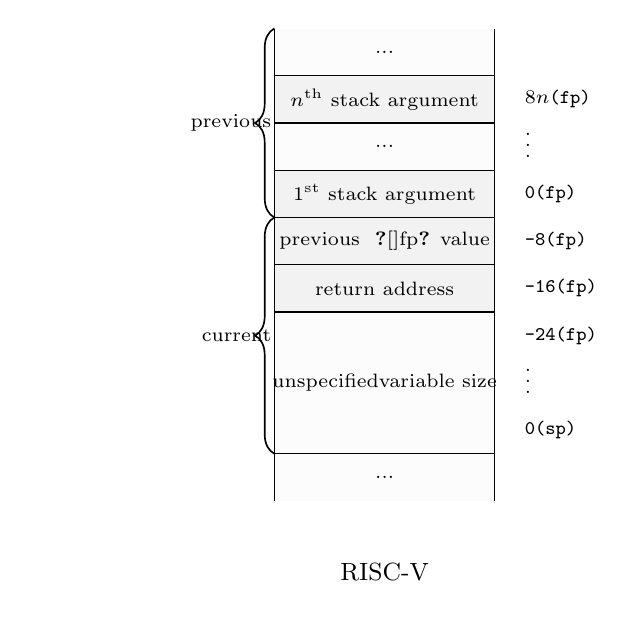
\begin{tikzpicture}[xscale=0.7, yscale=0.6]
			\scriptsize

			% manually set counter to allow stack frame including the start dots
			\setcounter{cellnb}{0}
			\startframe
			\addtocounter{cellnb}{-1}

			% copied code from `\stacktop{}` to not reset counter to in turn allow `\startframe` above this
			\draw[padding] (0,\value{cellnb})
			+(-2,.5) -- +(-2,-.5) -- +(2,-.5) -- +(2,.5);
			\draw (0,\value{cellnb}) node{...};

			\cell{$n$\textsuperscript{th} stack argument} \cellcom{\texttt{$8n$(fp)}}
			\cell[padding]{...}
			% custom draw instead of `\cellcom` for yshift
			\draw (2.4,\value{cellnb}) node[anchor=west, yshift=3.5pt] {\vdots};
			\cell{\nth{1} stack argument} \cellcom{\texttt{0(fp)}}
			\finishframe{previous}

			\startframe
			\cell{previous \qVerb{fp} value} \cellcom{\texttt{-8(fp)}}
			\cell{return address} \cellcom{\texttt{-16(fp)}}

			\padding{3}{\makecell{unspecified\\variable size}} \cellcom{\texttt{0(sp)}}
			% custom draws instead of `\cellcom` for yshift and padding cell offset
			\draw (2.4,\value{cellnb}+1) node[anchor=west, yshift=3.5pt] {\vdots};
			\draw (2.4,\value{cellnb}+2) node[anchor=west] {\texttt{-24(fp)}};
			\finishframe{current}
			\stackbottom[padding]

            \small
            \draw (0,\value{cellnb}-2)  node(currentcell) {\riscv{}};
		\end{tikzpicture}
	\end{minipage}
	\hfill
	\begin{minipage}{0.45\textwidth}
        \hspace{-2.75cm}
		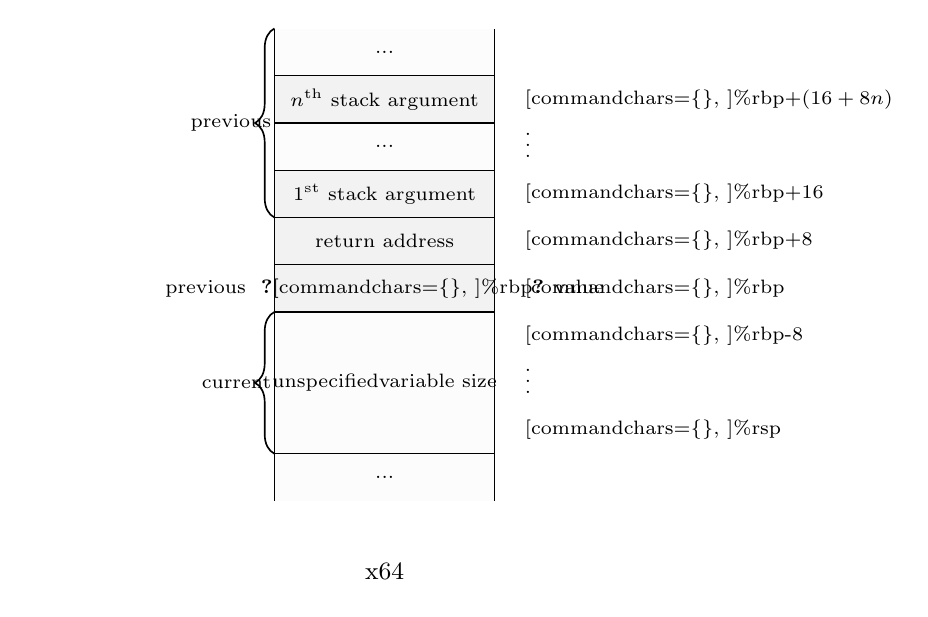
\begin{tikzpicture}[xscale=0.7, yscale=0.6]
			\scriptsize

			% manually set counter to allow stack frame including the start dots
			\setcounter{cellnb}{0}
			\startframe
			\addtocounter{cellnb}{-1}

			% copied code from `\stacktop{}` to not reset counter to in turn allow `\startframe` above this
			\draw[padding] (0,\value{cellnb})
			+(-2,.5) -- +(-2,-.5) -- +(2,-.5) -- +(2,.5);
			\draw (0,\value{cellnb}) node{...};

			\cell{$n$\textsuperscript{th} stack argument} \cellcom{\VerbCmd{\%rbp+}$(16+8n)$}
			\cell[padding]{...}
			% custom draw instead of `\cellcom` for yshift
			\draw (2.4,\value{cellnb}) node[anchor=west, yshift=3.5pt] {\vdots};
			\cell{\nth{1} stack argument} \cellcom{\VerbCmd{\%rbp+16}}
			\finishframe{previous}

			\cell{return address} \cellcom{\VerbCmd{\%rbp+8}}
			\cell{previous \qreg{rbp} value} \cellcom{\VerbCmd{\%rbp}}

			\startframe
			\padding{3}{\makecell{unspecified\\variable size}} \cellcom{\VerbCmd{\%rsp}}
			% custom draws instead of `\cellcom` for yshift and padding cell offset
			\draw (2.4,\value{cellnb}+1) node[anchor=west, yshift=3.5pt] {\vdots};
			\draw (2.4,\value{cellnb}+2) node[anchor=west] {\VerbCmd{\%rbp-8}};
			\finishframe{current}
			\stackbottom[padding]

            \small
            \draw (0,\value{cellnb}-2)  node(currentcell) {x64};
		\end{tikzpicture}
	\end{minipage}
\end{frame}

% LTeX: language=de-DE
% chktex-file -2
\section{Kompilierung zu \riscv}
\begin{frame}{Was ist \riscv?}
	\pdfpcnote{
		- RISC -> Reduced Instruction Set Computer
		- Forschungsprojekt der UC Berkeley
		- Lösen der Probleme von anderen Architekturen
		- Simplizit und Erweiterbarkeit
		- Unterstützt durch
		- Google
		- Microsoft
		- Samsung
		- IBM
	}

	\begin{itemize}
		\item<1-> \textbf{R}educed \textbf{I}nstruction \textbf{S}et \textbf{C}omputer (\cemph{RISC})
		\item<2-> \cemph{Forschungsprojekt} der UC Berkeley
		\item<3-> Lösen der Probleme vieler anderer Architekturen
		\item<4-> \cemph{Simplizität} und Erweiterbarkeit
		\item<5-> Unterstüztung durch: Google, Microsoft, Samsung und IBM
	\end{itemize}
\end{frame}

\begin{frame}{Beispiel}
	\begin{minipage}{0.4\textwidth}
		\vspace{.5cm}
		\Lirsting[float=H, fancyvrb={frame=none, fontsize=\small}]{deps/paper/listings/fib.rush}
		\centering
		\vspace{-.5cm}
		\Larrow{Ausgabe}
	\end{minipage}
	\hfill
	\begin{minipage}{0.4\textwidth}
		\Lirsting[float=H, fancyvrb={frame=none, fontsize=\scriptsize}, ranges={1-13, 28-40}]{listings/generated/fib_riscv.s}
	\end{minipage}
\end{frame}

\begin{frame}{Fazit zu \riscv}
	\begin{table}[h]
		\rowcolors{2}{gray!15}{}
		\begin{tabularx}{0.95\textwidth}{L|L}
			\cellcolor{green!20} Vorteile                       & \cellcolor{red!20} Nachteile        \\
			\hline
			Sehr neu und modern                                 & Geringe Verbreitung                 \\
			Komplett open-source und Gemeinschaftlich verwaltet & Eher experimentell                  \\
			Sehr übersichtliche und simple Architektur          & Einige Operationen sind aufwendiger \\
			Sehr gute und übersichtliche Dokumentation          & Weniger Online-Ressourcen           \\
		\end{tabularx}
	\end{table}
\end{frame}

% LTeX: language=de-DE
% chktex-file -2
\section{Kompilierung zu x86\_64}
\begin{frame}{Was ist x86\_64}
	\begin{itemize}
		\item<1-> Häufig auch x84-64 oder x64 genannt
		\item<2-> \textbf{C}omplex \textbf{I}instruction \textbf{S}et \textbf{C}omputer (CISC)
			\begin{itemize}
				\item<3-> Um vielfaches mehr Instruktionen als RISC Architekturen
			\end{itemize}
		\item<4-> Sehr weit verbreitet
	\end{itemize}
\end{frame}

\begin{frame}{Beispiel Ein-/Ausgabe}
	\pdfpcnote{
		- auch wieder dasselbe Fibonacci Beispiel \\
		- Ausgabe ist Asseembly (wie bei RISC-V) \\
		- aber ein anderes Assembly \\
		- es gibt verschiedene Assembly Dialekte, wir nutzen Intel Syntax \\
	}

	\begin{minipage}{0.45\textwidth}
		\Lirsting[float=H, fancyvrb={frame=none, fontsize=\small}]{deps/paper/listings/fib.rush}
		\centering
		\Larrow{Ausgabe}
	\end{minipage}
	\hfill
	\begin{minipage}{0.45\textwidth}
		\Lirsting[float=H, ranges={6-28, 39-42}, fancyvrb={frame=none, fontsize=\scriptsize}]{listings/generated/fib_x64.s}
	\end{minipage}
\end{frame}

\newcommand{\colregr}[1]{\textcolor[HTML]{e45649}{\Verb{#1}}}
\newcommand{\colregx}[1]{\textcolor[HTML]{e45649}{\reg{#1}}}
\begin{frame}{Vergleich mit \riscv{} Assembly}
	\pdfpcnote{
		1. Aufbau und Benennung von Instruktionen \\
		2. Benennung von Registern \\
		3. Syntax fuer Pointer \\
		4. Groesse eines Worts, und damit die Benennung der anderen Groessen \\
	}

	\centering
	\rowcolors{2}{gray!15}{}
	\begin{tabular}{l|l|l}
		\rowcolor{gray!20} Merkmal & \riscv{}                                                                                                                                                         & x64                                                                                                                                                                                                                                                                      \\
		\hline
		% NOTE: some lirstings are written without `\LirstInline` to have correct highlighting without
		% the missing context and to allow for `%` signs
		Instruktionen              & \LirstInline{asm}{addi a0, a0, 3}                                                                                                                                & \Verb[commandchars=\\\{\}]{\textcolor[HTML]{4078f2}{add} \textcolor[HTML]{e45649}{\%rax}\textcolor[HTML]{818387}{,} \textcolor[HTML]{c18401}{3}}                                                                                            \pause \\
		Register                   & \colregr{a0}, \colregr{a1}, \colregr{fa0}, \colregr{sp}, \dots                                                                                                   & \colregx{rax}, \colregx{rdi}, \colregx{xmm0}, \colregx{rsp}, \dots                                                                                                                                             \pause                                                    \\
		Pointer                    & \Verb[commandchars=\\\{\}]{\textcolor[HTML]{c18401}{-1}\textcolor[HTML]{818387}{(}\textcolor[HTML]{e45649}{fp}\textcolor[HTML]{818387}{)}} & \Verb[commandchars=\\\{\}]{\textcolor[HTML]{a626a4}{byte} \textcolor[HTML]{a626a4}{ptr} \textcolor[HTML]{818387}{[}\textcolor[HTML]{e45649}{\%rbp}\textcolor[HTML]{383a42}{-}\textcolor[HTML]{c18401}{1}\textcolor[HTML]{818387}{]}} \pause        \\
		Größe eines \emph{Wort}s   & 4 Byte                                                                                                                                                           & 2 Byte                                                                                                                                                                                                                                                                   \\
	\end{tabular}
\end{frame}

\begin{frame}{Fazit zu x64}
	\begin{table}[h]
		\rowcolors{2}{gray!15}{}
		\begin{tabular}{p{6cm}|p{6cm}}
			\cellcolor{green!20} Vorteile         & \cellcolor{red!20} Nachteile                 \\
			\hline
			Höherer Abstraktionsgrad als \riscv{} & Kompliziertere Übersetzung von z.B. Division \\
			Weite Verbreitung                     & Sehr alt und unübersichtlich                 \\
			Viele Online-Ressourcen               & Weniger übersichtliche Dokumentation         \\
		\end{tabular}
	\end{table}
\end{frame}

% LTeX: language=de-DE
\begin{frame}{Vergleich mit high-level Zielen}
	\begin{itemize}
		\item Deutlich anspruchsvoller
		\item Signifikanter Lernaufwand
		\item Detailliertes Verständnis notwendig
		\item Sehr fehleranfällig
		\item Benötigt keine direkten Abhängigkeiten
	\end{itemize}
\end{frame}

\section{Finale Anmerkungen \& Fazit}
\begin{frame}{Wir haben gelernt \dots}
	\pdfpcnote{
		@Mik \\
		\\
		1. Vertiefung \\
            - Lexer und Parser \\
            - Tree-walking interpreter (Pointer) \\
		\\
		--- \\
		\\
		2. Pratt Parsing \\
		3. Grundlagen anhand LLVM und WebAssembly \\
		4. low-level Programmierung und Assembly \\
	}
	\begin{itemize}
		\item<1-> Vertiefung
			\begin{itemize}
				\item <2-> Lexer und Parser
				\item <3-> Tree-walking Interpreter
			\end{itemize}
		\item<4-> Pratt Parsing
		\item<5-> LLVM und WebAssembly
		\item<6-> Assembly und low-level Programmierung
	\end{itemize}
\end{frame}

\begin{frame}{Links}
	\pdfpcnote{
		@Mik \\
		\\
		1. Uebersicht ueber rush: **Website** \\
		2. Neuste Version der Arbeit unter **paper** Subdomain \\
		3. Interaktiv eigene Programme unter der **play** subdomain \\
		4. Quelltext aller 17 oeffentlichen Projekte auf GitHub \\
		\\
		--- \\
		\\
		- Danke! \\
	}
	\centering
	\begin{minipage}{.5\textwidth}
		\begin{description}
			\item<1->[rush Website] \url{https://rush-lang.de}
			\item<2->[Paper] \url{https://paper.rush-lang.de}
			\item<3->[Playground] \url{https://play.rush-lang.de}
			\item<4->[GitHub] \url{https://github.com/rush-rs}
		\end{description}
	\end{minipage}
\end{frame}


% \listoffigures
% \listoftables
% \listof{listing}{Programmblockverzeichnis}
% \nocite{*}

\begin{frame}[shrink=30]
	\frametitle{Quellenverzeichnis}
    \vspace{1cm}
    \small\printbibliography[heading=bibintoc]
\end{frame}
\end{document}
